\subsection*{la fonction \textit{TD\_trier(int * T)}}
\subsubsection*{présentation}

La fonction \textit{TD\_trier(\dots)} initialise les indices de début et de fin du tri, et appelle la fonction \textit{tri\_pivot(\dots)} avec ces indices et les paramètres de base concernant les processeurs possédant le premier et le dernier élément à trier, la communication existante entre les processeurs, et leur rang. Tous ces paramètres sont utiles pour traiter le cas particulier d'une parallélisation des appels récursifs dont nous parlerons plus loin.

\begin{figure}[ht]
\centering
\caption*{Schéma de pré-tri}
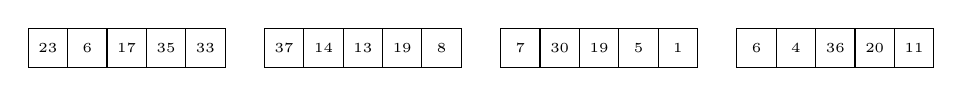
\begin{tikzpicture}[scale=0.5]
%%%%%%%%%%%%%%%%%%%%%%%%%%%%%%%%%%%%%%%%%%%%%%%%%%%%%%%%
% STYLE
\tikzstyle{case}=[rectangle,draw,minimum width=0.5cm,minimum height=0.5cm, font=\tiny]
\tikzstyle{op}=[circle,draw]
\tikzstyle{txt}=[]

\tikzset{link/.style={->,>=stealth'}}

%%%%%%%%%%%%%%%%%%%%%%%%%%%%%%%%%%%%%%%%%%%%%%%%%%%%%%%%
% NODES
\node[case] (T00) at (0, 0) {$23$};
\node[case] (T01) at (1, 0) {$6$};
\node[case] (T02) at (2, 0) {$17$};
\node[case] (T03) at (3, 0) {$35$};
\node[case] (T04) at (4, 0) {$33$};

\node[case] (T06) at (6, 0) {$37$};
\node[case] (T07) at (7, 0) {$14$};
\node[case] (T08) at (8, 0) {$13$};
\node[case] (T09) at (9, 0) {$19$};
\node[case] (T10) at (10, 0) {$8$};

\node[case] (T12) at (12, 0) {$7$};
\node[case] (T13) at (13, 0) {$30$};
\node[case] (T14) at (14, 0) {$19$};
\node[case] (T15) at (15, 0) {$5$};
\node[case] (T16) at (16, 0) {$1$};

\node[case] (T18) at (18, 0) {$6$};
\node[case] (T19) at (19, 0) {$4$};
\node[case] (T20) at (20, 0) {$36$};
\node[case] (T21) at (21, 0) {$20$};
\node[case] (T22) at (22, 0) {$11$};


%%%%%%%%%%%%%%%%%%%%%%%%%%%%%%%%%%%%%%%%%%%%%%%%%%%%%%%%
% LINKS

\end{tikzpicture}
\end{figure}

La fonction \textit{tri\_pivot(\dots)} est récursive. Le processeur désigné comme "processeur début" récupère la valeur de la première case à trier, qui fera office de pivot, et la distibue aux autres processeurs par l'utilisation de la fonction \verb+MPI_Bcast()+.
Par la suite, chaque processeur dans la communication fait appel à la fonction \textit{sort\_pivot(\dots)}, qui va leur permettre de chacun trier sa propre partie du tableau en fonction du pivot et de renvoyer l'indice de séparation (qui indique la première valeur supérieure ou égale au pivot).

\begin{figure}[ht]
\centering
\caption*{Schéma post-sort\_pivot pour $pivot = 23$}
\begin{tikzpicture}[scale=0.5]
%%%%%%%%%%%%%%%%%%%%%%%%%%%%%%%%%%%%%%%%%%%%%%%%%%%%%%%%
% STYLE
\tikzstyle{case}=[rectangle,draw,minimum width=0.5cm,minimum height=0.5cm, font=\tiny]
\tikzstyle{op}=[circle,draw]
\tikzstyle{txt}=[]

\tikzset{link/.style={->,>=stealth'}}

%%%%%%%%%%%%%%%%%%%%%%%%%%%%%%%%%%%%%%%%%%%%%%%%%%%%%%%%
% NODES
\node[case] (T00) at (0, 0) {$17$};
\node[case] (T01) at (1, 0) {$6$};
\node[case] (T02) at (2, 0) {$23$};
\node[case] (T03) at (3, 0) {$35$};
\node[case] (T04) at (4, 0) {$33$};

\node[case] (T06) at (6, 0) {$8$};
\node[case] (T07) at (7, 0) {$14$};
\node[case] (T08) at (8, 0) {$13$};
\node[case] (T09) at (9, 0) {$19$};
\node[case] (T10) at (10, 0) {$37$};

\node[case] (T12) at (12, 0) {$7$};
\node[case] (T13) at (13, 0) {$1$};
\node[case] (T14) at (14, 0) {$19$};
\node[case] (T15) at (15, 0) {$5$};
\node[case] (T16) at (16, 0) {$30$};

\node[case] (T18) at (18, 0) {$6$};
\node[case] (T19) at (19, 0) {$4$};
\node[case] (T20) at (20, 0) {$11$};
\node[case] (T21) at (21, 0) {$20$};
\node[case] (T22) at (22, 0) {$36$};


%%%%%%%%%%%%%%%%%%%%%%%%%%%%%%%%%%%%%%%%%%%%%%%%%%%%%%%%
% LINKS
\draw[link] (2,1) -> (T02);
\draw[link] (10,1) -> (T10);
\draw[link] (16,1) -> (T16);
\draw[link] (22,1) -> (T22);

\end{tikzpicture}
\end{figure}

La fonction \textit{swap(\dots)} est ensuite utilisée pour que les processeurs des parties "basses" du tableau et ceux des parties "hautes", s'échangent des valeurs qui sont trop grandes ou trop petites par rapport au pivot. Elle retourne l'indice du tableau marquant la séparation entre les éléments strictement inférieurs, et les éléments supérieurs au pivot.

\begin{figure}[ht]
\centering
\caption*{Schéma post-swap pour $pivot = 23$}
\begin{tikzpicture}[scale=0.5]
%%%%%%%%%%%%%%%%%%%%%%%%%%%%%%%%%%%%%%%%%%%%%%%%%%%%%%%%
% STYLE
\tikzstyle{case}=[rectangle,draw,minimum width=0.5cm,minimum height=0.5cm, font=\tiny]
\tikzstyle{op}=[circle,draw]
\tikzstyle{txt}=[]

\tikzset{link/.style={->,>=stealth'}}

%%%%%%%%%%%%%%%%%%%%%%%%%%%%%%%%%%%%%%%%%%%%%%%%%%%%%%%%
% NODES
\node[case] (T00) at (0, 0) {$17$};
\node[case] (T01) at (1, 0) {$6$};
\node[case] (T02) at (2, 0) {$20$};
\node[case] (T03) at (3, 0) {$11$};
\node[case] (T04) at (4, 0) {$4$};

\node[case] (T06) at (6, 0) {$8$};
\node[case] (T07) at (7, 0) {$14$};
\node[case] (T08) at (8, 0) {$13$};
\node[case] (T09) at (9, 0) {$19$};
\node[case] (T10) at (10, 0) {$6$};

\node[case] (T12) at (12, 0) {$7$};
\node[case] (T13) at (13, 0) {$1$};
\node[case] (T14) at (14, 0) {$19$};
\node[case] (T15) at (15, 0) {$5$};
\node[case] (T16) at (16, 0) {$30$};

\node[case] (T18) at (18, 0) {$37$};
\node[case] (T19) at (19, 0) {$33$};
\node[case] (T20) at (20, 0) {$35$};
\node[case] (T21) at (21, 0) {$23$};
\node[case] (T22) at (22, 0) {$36$};

\node[txt] (txt0) at (16, 2) {\tiny indice de séparation};
\node[txt] (txt1) at (15.5, -2) {\tiny séparation};
%%%%%%%%%%%%%%%%%%%%%%%%%%%%%%%%%%%%%%%%%%%%%%%%%%%%%%%%
% LINKS
\draw[link] (txt0) -> (T16);
\draw (15.5, 1) -> (15.5, -1);

\end{tikzpicture}
\end{figure}

Si l'indice récupéré indique juste le début de la partie d'un des processeurs, les deux sous tableaux à traiter sont gérés par 2 groupes de processeurs bien distincts, et on peut donc paralléliser.
Pour cela, on utilise la fonction \verb+MPI_Comm_split()+ pour séparer les processeurs de la communication actuelle dans 2 nouveaux groupes de communication. Le premier traitera la première sous-partie du tableau, et le deuxième traitera la deuxième. 

\cleardoublepage
Cela implique d'entrer en paramètre de la fonction \textit{tri\_pivot(\dots)} : la nouvelle communication, le rang du processeur dans la nouvelle communication, et les numéros des processeurs "debut" et "fin" dans la nouvelle communication.
Si l'indice récupéré est le même que le précédent ayant engendré une parallélisation, cela veut dire que les processeurs gérant la deuxième partie ont eu pour pivot le plus petit élément des éléments qu'ils ont à traiter, et qu'ils ne doivent pas tenter de paralléliser à nouveau, mais de travailler sur le même sous tableau moins le premier élément.

\begin{figure}[ht]
\centering
\caption*{Schéma cas parallélisation}
\begin{tikzpicture}[scale=0.5]
%%%%%%%%%%%%%%%%%%%%%%%%%%%%%%%%%%%%%%%%%%%%%%%%%%%%%%%%
% STYLE
\tikzstyle{case}=[rectangle,draw,minimum width=0.5cm,minimum height=0.5cm,font=\tiny]
\tikzstyle{op}=[circle,draw]
\tikzstyle{txt}=[]

\tikzset{link/.style={->,>=stealth'}}

%%%%%%%%%%%%%%%%%%%%%%%%%%%%%%%%%%%%%%%%%%%%%%%%%%%%%%%%
% NODES
\node[case] (T00) at (0, 0) {$4$};
\node[case] (T01) at (1, 0) {$6$};
\node[case] (T02) at (2, 0) {$11$};
\node[case] (T03) at (3, 0) {$5$};
\node[case] (T04) at (4, 0) {$1$};

\node[case] (T06) at (6, 0) {$8$};
\node[case] (T07) at (7, 0) {$14$};
\node[case] (T08) at (8, 0) {$13$};
\node[case] (T09) at (9, 0) {$6$};
\node[case] (T10) at (10, 0) {$7$};

\node[case] (T12) at (14, 0) {$19$};
\node[case] (T13) at (15, 0) {$17$};
\node[case] (T14) at (16, 0) {$20$};
\node[case] (T15) at (17, 0) {$19$};
\node[case] (T16) at (18, 0) {};

\node[case] (T20) at (20, 0) {};
\node[case] (T21) at (21, 0) {};
\node[case] (T22) at (22, 0) {};
\node[case] (T23) at (23, 0) {};
\node[case] (T24) at (24, 0) {};

\node[txt] (txt0) at (2,-1) {\tiny proc1};
\node[txt] (txt1) at (8,-1) {\tiny proc2};
\node[txt] (txt2) at (16,-1) {\tiny proc3};
\node[txt] (txt3) at (22,-1) {\tiny proc4};

\node[txt] (txt4) at (5,-2) {\tiny comm1};
\node[txt] (txt5) at (19,-2) {\tiny comm2};

\node[txt] (txt6) at (14,1.5) {\tiny indice de séparation};

\node[txt] (txt2) at (5, 3.2) {\tiny tri sur ce tableau};
\node[txt] (txt2) at (15.5, 3.2) {\tiny tri sur ce tableau};

%%%%%%%%%%%%%%%%%%%%%%%%%%%%%%%%%%%%%%%%%%%%%%%%%%%%%%%%
% LINKS
\draw (11.9,1) -- (11.9,-1);
\draw (12.1,1) -- (12.1,-1);
\draw[link] (txt6) -- (T12);

\draw[
    decorate,
    decoration={brace,amplitude=10pt,mirror}
    ] 
    (0,-1) -- (10,-1);
            
\draw[
    decorate,
    decoration={brace,amplitude=10pt,mirror},
    ] 
    (14,-1) -- (24,-1);
    
\draw[
    decorate,
    decoration={brace,amplitude=10pt}
    ] 
    (0,2) -- (10,2);
            
\draw[
    decorate,
    decoration={brace,amplitude=10pt}
    ] 
    (14,2) -- (17,2);

\end{tikzpicture}
\end{figure}

Si on ne peut pas paralléliser, on appelle, de la même manière, la fonction \textit{tri\_pivot(\dots)} sur le premier sous-tableau, on attend la fin de son exécution, et on fait appel au tri sur la deuxième sous partie. On doit absolument attendre la fin du tri du premier sous tableau car le processeur qui possède le début du deuxième sous tableau sera occupé à trier le premier, et donc il y aura des incohérences dans les appels des fonctions de communication inter-processeurs.
A noter qu'avec la méthode où on parallélise, il est malheureusement impossible d'utiliser les fonctions \verb+MPI_Get()+ ou \verb+MPI_Put()+ pour récupérer le pivot ou échanger les valeurs, car pour cela, il faut que tous les processeurs appellent la fonction \verb+MPI_Win_fence+, et si le traitement d'un sous tableau est plus long que l'autre, il n'y aura pas le même nombre d'appels à cette fonction, et donc un problème de synchronisation.

\begin{figure}[ht]
\centering
\caption*{Schéma du cas sans parallélisation}
\begin{tikzpicture}[scale=0.5]
%%%%%%%%%%%%%%%%%%%%%%%%%%%%%%%%%%%%%%%%%%%%%%%%%%%%%%%%
% STYLE
\tikzstyle{case}=[rectangle,draw,minimum width=0.5cm,minimum height=0.5cm,font=\tiny]
\tikzstyle{op}=[circle,draw]
\tikzstyle{txt}=[]

\tikzset{link/.style={->,>=stealth'}}

%%%%%%%%%%%%%%%%%%%%%%%%%%%%%%%%%%%%%%%%%%%%%%%%%%%%%%%%
% NODES
\node[txt] (txt2) at (7.5, 2.6) {\tiny tri sur ce tableau};
\node[txt] (txt6) at (-2, 0) {\tiny (étape $1$)};
\node[txt] (txt7) at (-2, -3) {\tiny (étape $2$)};

\node[case] (T00) at (0, 0) {$17$};
\node[case] (T01) at (1, 0) {$6$};
\node[case] (T02) at (2, 0) {$20$};
\node[case] (T03) at (3, 0) {$11$};
\node[case] (T04) at (4, 0) {$4$};

\node[case] (T06) at (6, 0) {$8$};
\node[case] (T07) at (7, 0) {$14$};
\node[case] (T08) at (8, 0) {$13$};
\node[case] (T09) at (9, 0) {$19$};
\node[case] (T10) at (10, 0) {$6$};

\node[case] (T12) at (12, 0) {$7$};
\node[case] (T13) at (13, 0) {$1$};
\node[case] (T14) at (14, 0) {$19$};
\node[case] (T15) at (15, 0) {$5$};
\node[case] (T23) at (16, 0) {};

\node[case] (T25) at (18, 0) {};
\node[case] (T26) at (19, 0) {};
\node[case] (T27) at (20, 0) {};
\node[case] (T28) at (21, 0) {};
\node[case] (T29) at (22, 0) {};

\node[txt] (txt5) at (11, -1.5) {\tiny \textbf{MPI\_Barrier(comm)}};

\node[case] (T30) at (0, -3) {};
\node[case] (T31) at (1, -3) {};
\node[case] (T32) at (2, -3) {};
\node[case] (T33) at (3, -3) {};
\node[case] (T34) at (4, -3) {};

\node[case] (T36) at (6, -3) {};
\node[case] (T37) at (7, -3) {};
\node[case] (T38) at (8, -3) {};
\node[case] (T39) at (9, -3) {};
\node[case] (T40) at (10, -3) {};

\node[case] (T42) at (12, -3) {};
\node[case] (T43) at (13, -3) {};
\node[case] (T44) at (14, -3) {};
\node[case] (T45) at (15, -3) {};
\node[case] (T53) at (16, -3) {$30$};

\node[case] (T55) at (18, -3) {$37$};
\node[case] (T56) at (19, -3) {$33$};
\node[case] (T57) at (20, -3) {$35$};
\node[case] (T58) at (21, -3) {$23$};
\node[case] (T59) at (22, -3) {$36$};

\node[txt] (txt3) at (19, -5.6) {\tiny tri sur ce tableau};

\node[txt] (txt0) at (0, 1) {\tiny début};
\node[txt] (txt1) at (15, 1) {\tiny fin};

\node[txt] (txt10) at (16, -4) {\tiny début};
\node[txt] (txt11) at (22, -4) {\tiny fin};

%%%%%%%%%%%%%%%%%%%%%%%%%%%%%%%%%%%%%%%%%%%%%%%%%%%%%%%%
% LINKS
\draw[link] (txt0) -- (T00);
\draw[link] (txt1) -- (T15);
\draw[link] (txt10) -- (T53);
\draw[link] (txt11) -- (T59);

\draw[
    decorate,
    decoration={brace,amplitude=10pt}
    ] 
    (0,1.5) -- (15,1.5);
    
\draw[
    decorate,
    decoration={brace,amplitude=10pt,mirror}
    ] 
    (16,-4.5) -- (22,-4.5);

\end{tikzpicture}
\end{figure}

On a donc le code ci-dessous :
\lstinputlisting[language=c, style=b&w, title={La fonction \textit{tri\_pivot(\dots)} abrégée}]{listings/tri-pivot.c}

\subsubsection*{la fonction \textit{sort\_pivot(\dots)}}
La fonction \textit{sort\_pivot(\dots)} effectue un tri rapide sur ses éléments par rapport au pivot entré en paramètre. Deux indices sont initialisés aux indices de début et de fin de tri de la portion du processeur en question. L'indice de début est incrémenté tant qu'on trouve des valeurs inférieures strictement au pivot, puis l'indice de fin est décrémenté tant qu'on trouve des valeurs supérieures ou égales au pivot. Si l'indice de début est inférieur à l'indice de fin, on fait l'échange, sinon on arrête. On recommence tant que l'indice de début est strictement inférieur à celui de fin.
Enfin l'indice renvoyé est l'indice de début, qui aura été incrémenté une fois de plus si la valeur sur laquelle il pointe est strictement inférieure au pivot, ce qui veut dire que tous les éléments gérés par le processeur sont strictement inférieurs au pivot.

On a donc le code ci-dessous :
\lstinputlisting[language=c, style=b&w, title={La fonction \textit{sort\_pivot(\dots)} abrégée}]{listings/sort-pivot.c}

\cleardoublepage
\subsubsection*{la fonction \textit{swap(\dots)}}
Dans cette fonction, un processeur est initialement le "processeur de début", et un autre est le "processeur de fin". Tant que le premier est strictement inférieur au deuxième, on n'a pas terminé le traitement. Pour ce traitement, on vérifie que le "processeur de début" a une valeur à échanger (c'est-à-dire strictement inférieure au pivot), c'est le cas si son indice (récupéré grâce à la fonction \textit{sort\_pivot(\dots)}) est inférieur ou égal à l'indice de son dernier élément. Un booléen "deb\_valide" est modifié pour indiquer si oui ou non le "processeur de début" a une valeur à échanger. Ce booléen est envoyé aux autres processeurs de la communication par un broadcast. S'il est à 0, tout le monde incrémente son numéro du "processeur de début", s'il est à 1, le "processeur de fin" fait de même (il vérifie que son indice est supérieur stricement à l'indice de son premier élément, modifie son booléen "fin\_valide", et le broadcast à tous les processeurs de la communication). S'il a également une valeur à échanger, on effectue l'échange grâce à des \verb+MPI_Recv()+ et \verb+MPI_Send()+, puis l'indice du "processeur de début" est incrémenté, et celui du "processeur de fin" est décrémenté. S'il n'a pas de valeur à échanger, on recommence.
A chaque début de la boucle, les processeurs vérifient s'ils sont le processeur de début, puis, plus loin, s'ils sont le processeur de fin.
Lorsque le numéro du "processeur de début" n'est plus strictement inférieur à celui du "processeur de fin", on arrête. Il reste à déterminer lequel du "processeur de début" ou du "processeur de fin" doit fournir l'indice qui permet de séparer le tableau en deux. On fait cela grace à un booléen "last\_move" qui est mis à 0 lorsque le numéro du "processeur de début" avance, ou à 1 lorsque celui du "processeur de fin" est décrémenté. A la fin du traitement, on sait donc lequel à été changé en dernier, et on sait que l'autre peut posséder des valeurs inférieures et supérieures au pivot, c'est donc cet autre processeur qui fait un broadcast de l'indice à rapporter. Cet indice est la valeur de retour de la fonction \textit{swap(\dots)}, il indique la séparation en deux du tableau.

On a donc le code ci-dessous :
\lstinputlisting[language=c, style=b&w, title={La fonction \textit{swap(\dots)} abrégée}]{listings/swap.c}

\cleardoublepage
\subsubsection*{exemple d'exécution du \textit{swap}}

\begin{itemize}
\item \textbf{étape 0}

\begin{center}
\begin{tikzpicture}[scale=0.5]
%%%%%%%%%%%%%%%%%%%%%%%%%%%%%%%%%%%%%%%%%%%%%%%%%%%%%%%%
% STYLE
\tikzstyle{case}=[rectangle,draw,minimum width=0.5cm,minimum height=0.5cm, font=\tiny]
\tikzstyle{op}=[circle,draw]
\tikzstyle{txt}=[font=\tiny]

\tikzset{link/.style={->,>=stealth'}}

%%%%%%%%%%%%%%%%%%%%%%%%%%%%%%%%%%%%%%%%%%%%%%%%%%%%%%%%
% NODES
\node[case] (T00) at (0, 0) {$4$};
\node[case] (T01) at (1, 0) {$8$};
\node[case] (T02) at (2, 0) {$11$};
\node[case] (T03) at (3, 0) {$16$};

\node[case] (T06) at (6, 0) {$2$};
\node[case] (T07) at (7, 0) {$7$};
\node[case] (T08) at (8, 0) {$19$};
\node[case] (T09) at (9, 0) {$18$};

\node[case] (T12) at (12, 0) {$0$};
\node[case] (T13) at (13, 0) {$15$};
\node[case] (T14) at (14, 0) {$3$};
\node[case] (T15) at (15, 0) {$17$};
\node[case] (T16) at (16, 0) {$16$};

\node[txt] (txt0) at (3,1) {$indice = 3$};
\node[txt] (txt1) at (8,1) {$indice = 2$};
\node[txt] (txt2) at (15,1) {$indice = 3$};

\node[txt] (txt3) at (1.5,-1) {proc\_deb};
\node[txt] (txt4) at (14,-1) {proc\_fin};

\node[txt,align=left] (txt5) at (-3,0) {
$proc\_deb=0$\\
$proc\_fin=2$
};
%%%%%%%%%%%%%%%%%%%%%%%%%%%%%%%%%%%%%%%%%%%%%%%%%%%%%%%%
% LINKS
\draw[link] (txt0) -> (T03);
\draw[link] (txt1) -> (T08);
\draw[link] (txt2) -> (T15);
\end{tikzpicture}
\end{center}

\item \textbf{étape 1}

Les indices proc\_deb et proc\_fin sont valides, on échange et on modifie les indices.\\

\begin{center}
\begin{tikzpicture}[scale=0.5]
%%%%%%%%%%%%%%%%%%%%%%%%%%%%%%%%%%%%%%%%%%%%%%%%%%%%%%%%
% STYLE
\tikzstyle{case}=[rectangle,draw,minimum width=0.5cm,minimum height=0.5cm, font=\tiny]
\tikzstyle{op}=[circle,draw]
\tikzstyle{txt}=[font=\tiny]

\tikzset{link/.style={->,>=stealth'}}

%%%%%%%%%%%%%%%%%%%%%%%%%%%%%%%%%%%%%%%%%%%%%%%%%%%%%%%%
% NODES
\node[case] (T00) at (0, 0) {$4$};
\node[case] (T01) at (1, 0) {$8$};
\node[case] (T02) at (2, 0) {$11$};
\node[case] (T03) at (3, 0) {$3$};

\node[case] (T06) at (6, 0) {$2$};
\node[case] (T07) at (7, 0) {$7$};
\node[case] (T08) at (8, 0) {$19$};
\node[case] (T09) at (9, 0) {$18$};

\node[case] (T12) at (12, 0) {$0$};
\node[case] (T13) at (13, 0) {$15$};
\node[case] (T14) at (14, 0) {$16$};
\node[case] (T15) at (15, 0) {$17$};
\node[case] (T16) at (16, 0) {$16$};

\node[txt] (txt0) at (4,1) {$indice = 4$};
\node[txt] (txt1) at (8,1) {$indice = 2$};
\node[txt] (txt2) at (14,1) {$indice = 2$};

\node[txt] (txt3) at (1.5,-1) {proc\_deb};
\node[txt] (txt4) at (14,-1) {proc\_fin};

\node[txt,align=left] (txt5) at (-3,0) {
$proc\_deb=0$\\
$proc\_fin=2$
};
%%%%%%%%%%%%%%%%%%%%%%%%%%%%%%%%%%%%%%%%%%%%%%%%%%%%%%%%
% LINKS
\draw[link] (txt0) -> (4, 0.5);
\draw[link] (txt1) -> (T08);
\draw[link] (txt2) -> (T14);
\end{tikzpicture}
\end{center}

\item \textbf{étape 2}

L'indice de proc\_deb n'est pas bon, on incrémente proc\_deb et on recommence.

\begin{center}
\begin{tikzpicture}[scale=0.5]
%%%%%%%%%%%%%%%%%%%%%%%%%%%%%%%%%%%%%%%%%%%%%%%%%%%%%%%%
% STYLE
\tikzstyle{case}=[rectangle,draw,minimum width=0.5cm,minimum height=0.5cm, font=\tiny]
\tikzstyle{op}=[circle,draw]
\tikzstyle{txt}=[font=\tiny]

\tikzset{link/.style={->,>=stealth'}}

%%%%%%%%%%%%%%%%%%%%%%%%%%%%%%%%%%%%%%%%%%%%%%%%%%%%%%%%
% NODES
\node[case] (T00) at (0, 0) {$4$};
\node[case] (T01) at (1, 0) {$8$};
\node[case] (T02) at (2, 0) {$11$};
\node[case] (T03) at (3, 0) {$3$};

\node[case] (T06) at (6, 0) {$2$};
\node[case] (T07) at (7, 0) {$7$};
\node[case] (T08) at (8, 0) {$19$};
\node[case] (T09) at (9, 0) {$18$};

\node[case] (T12) at (12, 0) {$0$};
\node[case] (T13) at (13, 0) {$15$};
\node[case] (T14) at (14, 0) {$16$};
\node[case] (T15) at (15, 0) {$17$};
\node[case] (T16) at (16, 0) {$16$};

\node[txt] (txt1) at (8,1) {$indice = 2$};
\node[txt] (txt2) at (14,1) {$indice = 2$};

\node[txt] (txt3) at (7.5,-1) {proc\_deb};
\node[txt] (txt4) at (14,-1) {proc\_fin};

\node[txt,align=left] (txt5) at (-3,0) {
$proc\_deb=1$\\
$proc\_fin=2$
};
%%%%%%%%%%%%%%%%%%%%%%%%%%%%%%%%%%%%%%%%%%%%%%%%%%%%%%%%
% LINKS
\draw[link] (txt1) -> (T08);
\draw[link] (txt2) -> (T14);
\end{tikzpicture}
\end{center}

\item \textbf{étape 3}

Les indices sont bons, on échange et on modifie les indices.

\begin{center}
\begin{tikzpicture}[scale=0.5]
%%%%%%%%%%%%%%%%%%%%%%%%%%%%%%%%%%%%%%%%%%%%%%%%%%%%%%%%
% STYLE
\tikzstyle{case}=[rectangle,draw,minimum width=0.5cm,minimum height=0.5cm, font=\tiny]
\tikzstyle{op}=[circle,draw]
\tikzstyle{txt}=[font=\tiny]

\tikzset{link/.style={->,>=stealth'}}

%%%%%%%%%%%%%%%%%%%%%%%%%%%%%%%%%%%%%%%%%%%%%%%%%%%%%%%%
% NODES
\node[case] (T00) at (0, 0) {$4$};
\node[case] (T01) at (1, 0) {$8$};
\node[case] (T02) at (2, 0) {$11$};
\node[case] (T03) at (3, 0) {$3$};

\node[case] (T06) at (6, 0) {$2$};
\node[case] (T07) at (7, 0) {$7$};
\node[case] (T08) at (8, 0) {$15$};
\node[case] (T09) at (9, 0) {$18$};

\node[case] (T12) at (12, 0) {$0$};
\node[case] (T13) at (13, 0) {$19$};
\node[case] (T14) at (14, 0) {$16$};
\node[case] (T15) at (15, 0) {$17$};
\node[case] (T16) at (16, 0) {$16$};

\node[txt] (txt1) at (9,1) {$indice = 3$};
\node[txt] (txt2) at (13,1) {$indice = 1$};

\node[txt] (txt3) at (7.5,-1) {proc\_deb};
\node[txt] (txt4) at (14,-1) {proc\_fin};

\node[txt,align=left] (txt5) at (-3,0) {
$proc\_deb=1$\\
$proc\_fin=2$
};
%%%%%%%%%%%%%%%%%%%%%%%%%%%%%%%%%%%%%%%%%%%%%%%%%%%%%%%%
% LINKS
\draw[link] (txt1) -> (T09);
\draw[link] (txt2) -> (T13);
\end{tikzpicture}
\end{center}

\item \textbf{étape 4}

Les indices sont bons, on échange et on modifie les indices.

\begin{center}
\begin{tikzpicture}[scale=0.5]
%%%%%%%%%%%%%%%%%%%%%%%%%%%%%%%%%%%%%%%%%%%%%%%%%%%%%%%%
% STYLE
\tikzstyle{case}=[rectangle,draw,minimum width=0.5cm,minimum height=0.5cm, font=\tiny]
\tikzstyle{op}=[circle,draw]
\tikzstyle{txt}=[font=\tiny]

\tikzset{link/.style={->,>=stealth'}}

%%%%%%%%%%%%%%%%%%%%%%%%%%%%%%%%%%%%%%%%%%%%%%%%%%%%%%%%
% NODES
\node[case] (T00) at (0, 0) {$4$};
\node[case] (T01) at (1, 0) {$8$};
\node[case] (T02) at (2, 0) {$11$};
\node[case] (T03) at (3, 0) {$3$};

\node[case] (T06) at (6, 0) {$2$};
\node[case] (T07) at (7, 0) {$7$};
\node[case] (T08) at (8, 0) {$15$};
\node[case] (T09) at (9, 0) {$0$};

\node[case] (T12) at (12, 0) {$18$};
\node[case] (T13) at (13, 0) {$19$};
\node[case] (T14) at (14, 0) {$16$};
\node[case] (T15) at (15, 0) {$17$};
\node[case] (T16) at (16, 0) {$16$};

\node[txt] (txt1) at (10,1) {$indice = 4$};
\node[txt] (txt2) at (12,1.5) {$indice = 0$};

\node[txt] (txt3) at (7.5,-1) {proc\_deb};
\node[txt] (txt4) at (14,-1) {proc\_fin};

\node[txt,align=left] (txt5) at (-3,0) {
$proc\_deb=1$\\
$proc\_fin=2$
};
%%%%%%%%%%%%%%%%%%%%%%%%%%%%%%%%%%%%%%%%%%%%%%%%%%%%%%%%
% LINKS
\draw[link] (txt1) -> (10, 0.5);
\draw[link] (txt2) -> (T12);
\end{tikzpicture}
\end{center}

\item \textbf{étape 5}

L'indice de proc\_deb est faux, on incrémente proc\_deb.

\begin{center}
\begin{tikzpicture}[scale=0.5]
%%%%%%%%%%%%%%%%%%%%%%%%%%%%%%%%%%%%%%%%%%%%%%%%%%%%%%%%
% STYLE
\tikzstyle{case}=[rectangle,draw,minimum width=0.5cm,minimum height=0.5cm, font=\tiny]
\tikzstyle{op}=[circle,draw]
\tikzstyle{txt}=[font=\tiny]

\tikzset{link/.style={->,>=stealth'}}

%%%%%%%%%%%%%%%%%%%%%%%%%%%%%%%%%%%%%%%%%%%%%%%%%%%%%%%%
% NODES
\node[case] (T00) at (0, 0) {$4$};
\node[case] (T01) at (1, 0) {$8$};
\node[case] (T02) at (2, 0) {$11$};
\node[case] (T03) at (3, 0) {$3$};

\node[case] (T06) at (6, 0) {$2$};
\node[case] (T07) at (7, 0) {$7$};
\node[case] (T08) at (8, 0) {$15$};
\node[case] (T09) at (9, 0) {$0$};

\node[case] (T12) at (12, 0) {$18$};
\node[case] (T13) at (13, 0) {$19$};
\node[case] (T14) at (14, 0) {$16$};
\node[case] (T15) at (15, 0) {$17$};
\node[case] (T16) at (16, 0) {$16$};

\node[txt] (txt2) at (12,1) {$indice = 0$};

\node[txt] (txt3) at (14,-1) {proc\_deb et proc\_fin};

\node[txt,align=left] (txt5) at (-3,0) {
$proc\_deb=2$\\
$proc\_fin=2$
};
%%%%%%%%%%%%%%%%%%%%%%%%%%%%%%%%%%%%%%%%%%%%%%%%%%%%%%%%
% LINKS
\draw[link] (txt2) -> (T12);
\end{tikzpicture}
\end{center}

\item \textbf{étape 6}

On s'arrête et on broadcast l'indice de proc\_deb qui est $0$ ajouté à l'indice de début du block. La séparation pour les appels récursifs est donc la suivante :

\begin{center}
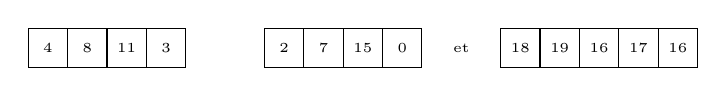
\begin{tikzpicture}[scale=0.5]
%%%%%%%%%%%%%%%%%%%%%%%%%%%%%%%%%%%%%%%%%%%%%%%%%%%%%%%%
% STYLE
\tikzstyle{case}=[rectangle,draw,minimum width=0.5cm,minimum height=0.5cm, font=\tiny]
\tikzstyle{op}=[circle,draw]
\tikzstyle{txt}=[font=\tiny]

\tikzset{link/.style={->,>=stealth'}}

%%%%%%%%%%%%%%%%%%%%%%%%%%%%%%%%%%%%%%%%%%%%%%%%%%%%%%%%
% NODES
\node[case] (T00) at (0, 0) {$4$};
\node[case] (T01) at (1, 0) {$8$};
\node[case] (T02) at (2, 0) {$11$};
\node[case] (T03) at (3, 0) {$3$};

\node[case] (T06) at (6, 0) {$2$};
\node[case] (T07) at (7, 0) {$7$};
\node[case] (T08) at (8, 0) {$15$};
\node[case] (T09) at (9, 0) {$0$};

\node[case] (T12) at (12, 0) {$18$};
\node[case] (T13) at (13, 0) {$19$};
\node[case] (T14) at (14, 0) {$16$};
\node[case] (T15) at (15, 0) {$17$};
\node[case] (T16) at (16, 0) {$16$};

\node[txt] (txt2) at (10.5,0) {et};
%%%%%%%%%%%%%%%%%%%%%%%%%%%%%%%%%%%%%%%%%%%%%%%%%%%%%%%%
% LINKS
\end{tikzpicture}
\end{center}

\end{itemize}

\cleardoublepage
\subsubsection*{analyse du tri}
Le tri appelle la fonction \textit{sort\_pivot(\dots)} dans laquelle chaque processeur parcourt toutes ses cases, on a donc un temps de $\frac{n}{p}$, la fonction swap parcourt toutes les cases concernées par un éventuel changement, en moyenne $\frac{n}{2}$ (si chaque processeur à autant de valeurs plus grandes que le processeur et plus petites, pour chaque processeur, seules la moitié de ces valeurs est parcrourue). Puis il y a les appels récursifs, qui peuvent être parallélisés dans un cas particulier (probabilité de $\frac{p}{n}$ d'être dans ce cas), ou pas dans tous les autres cas, dont on considère qu'en moyenne, ils découpent le tableau en $2$. 

On a donc une fonction qui a une équation de complexité : 
$$T(n) = 2 \times T(\frac{n}{2}) + c \times n$$

Où $c$ est une constante. L'algorithme prend donc un temps moyen en $\Theta (n \times log \, n)$ pour trier le tableau.








